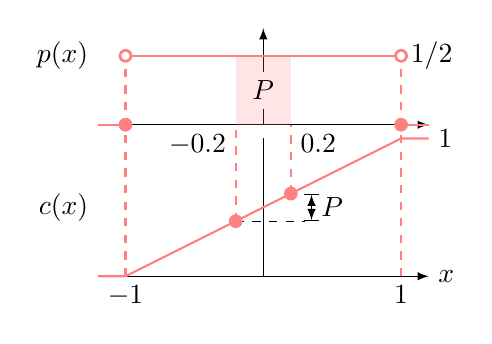
\begin{tikzpicture}[> = latex, scale=1.75]
    \def\r{0.05}
    % PDF
    %% Axis
    \draw [->] (-1.2, 0) -- (1.2, 0);
    \draw [->] (0, 0) -- (0, 0.7);
    %% Curve
    \fill [red!50, opacity=0.2]
        (-0.2, 0) rectangle (0.2, 0.5);
    \node [fill=red!10] at (0, 0.25) {$P$}; 
    \draw [thick, red!50] 
    (-1.2, 0) -- (-1, 0)
    (-1, 0.5) -- (1, 0.5) 
    (1, 0) -- (1.2, 0);
    %% Decorations
    \fill [red!50] 
        (-1, 0.5) circle (\r)
        (1, 0.5) circle (\r)
        (-1, 0) circle (\r)
        (1, 0) circle (\r);
    \fill [white] 
        (-1, 0.5) circle (\r-0.02)
        (1, 0.5) circle (\r-0.02);
    %% Annotations
    \draw 
        (1, 0.5) node [right] {$1/2$}
        (-0.2, 0) node [below left] {$-0.2$}
        (0.2, 0) node [below right] {$0.2$}
        (-1.2, 0.5) node [left] {$p(x)$};
        
    % CDF 
    \begin{scope}[shift={(0, -1.1)}]
    %% Axis
    \draw [->] (-1.2, 0) -- (1.2, 0) node [right] {$x$};
    \draw (0, 0) -- (0, 1);
    %% Curve
    \draw [thick, red!50] (-1.2, 0) -- (-1, 0) -- (1, 1) -- (1.2, 1);
    %% Decorations
    \draw [thick, red!50, dashed]
        (-1, 0) -- (-1, 0.5 +1.05)
        (1, 0) -- (1, 0.5 +1.05)
        (-0.2, 0.4) -- (-0.2, 1.1)
        (0.2, 0.6) -- (0.2, 1.1);
    %% Annotations
    \draw
        (-1, 0) node [below] {$-1$}
        (1, 0) node [below] {$1$}
        (1.2, 1) node [right] {$1$}
        (-1.2, 0.5) node [left] {$c(x)$};
    \draw [dashed] (-0.2, 0.4) --++ (0.5, 0);
    \fill [red!50] 
        (-0.2, 0.4) circle (\r)
        (0.2, 0.6) circle (\r);
    \draw [ |<->| ] (0.2 +0.15, 0.6) --++ (0, -0.2) node [midway, right] {$P$};
    \end{scope}
\end{tikzpicture}